\chapter{第二章\quad 项目意义及背景介绍}
\section{项目意义}
对电子商务任务调度模式下的异常监测的可视化实现,对此类控制平台提出了一种新的思路和方法,也是数据可视化在交叉领域的全新进展。
\subsection{电商集群的规模化}
2018年7月10日,2018中国互联网大会发布了新一版的《中国互联网发展报告(2018)》。报告中指出,2017年,中国电子商务交易服务营收规模为5027亿元,首次突破5000亿大关。2017年第三方互联网支付也达到143.26万亿,网络购物市场交易规模达5.33万亿元,而网络零售的市场交易规模为7.18万亿。中国网上支付用户规模达5.31亿人,其中手机支付用户就达5.27亿人,较2016年底增加5783万人,年增长率为12.3\%,规模增长迅速。正如网民在现实生活中体会到的,电子商务交易已经成为我们购买日常用品的首选手段,在中国庞大的网民基数和中国网络技术飞速发展的双重影响下,这一数字在以后还会以大增幅增长。根据商务部统计,2020年预计中国网络零售市场规模为9.6万亿,是2012年的10倍之多。电子商务在深度影响着国民生活的同时,也掌握着货架经济的命脉,倘若电商集群由于某种原因崩溃的话,给整个国家带来的影响即将是灾难性的。

中国电子商务的龙头企业——阿里巴巴网络技术有限公司(以下简称阿里巴巴),在国内的电子交易平台里扮演着举足轻重的地位。根据2018年阿里巴巴公布的财年财报显示:2018全年,阿里巴巴营收 2502.66 亿元人民币(约 398.98 亿美元),同比增长 58\%,核心电商业务收入 2140.20 亿元人民币,同比增长 60\%,均创下IPO(Initial Public Offerings,指股份公司首次向社会公众公开招股的发行方式,简称IPO)以来年度最高增幅,2018 财年净利润为 832.14 亿元人民币(约 132.66 亿美元)。如此庞大的交易额和成交额使专家和研究人员不自主地将目光放在其身上。2018年阿里巴巴在Github上公布了一组数据,该数据刻画了阿里巴巴在8天地范围内4000台服务器的运行状态的数据,而这组数据也将成为本项目的研究数据集,在本章第三部分,将会着重对该数据进行详细介绍。

\subsection{故障问题及手段}
电子商务平台的实现其实并不是一个不能达到的要求,但是任何系统架构在达到一定规模之后,大大小小的问题往往会接踵而至,而这也是一个企业生存的关键。2018年8月1日,阿里巴巴旗下的淘宝网交易平台,淘宝服务器出现大范围的故障,全国多地网友在微博反馈称自己的淘宝崩溃无法查看订单,淘宝App、PC版网页均出现“网络竟然崩溃了”的提示,即使切换网络和重启手机也无效,在长达数小时的等待之后,该漏洞得到了修复。具体的原因,阿里巴巴并没有给出明确的回复,之后这件事也就不了了之。然而这已经不是阿里巴巴遇到的第一次服务器崩溃事件,每隔数月就会时不时的发生类似的服务器故障。由此可见,即使是如此宏大的电子商务企业也会因为后端服务器的宕机事件,造成企业形象的不良影响的同时也造成了利润的亏损。换句话说,如果能快速发现故障,找出导致该进程异常的原因,再利用分支等手段同时进行维护,结果将会截然不同。而本系统的设计初衷就是以阻止此类问题的发生而提出的。
\subsection{设计优势}
本系统设计将基于可视分析,在对服务器异常进行图形化展示的同时,还拥有异常定位、时序性监测等特点,对出现异常信号的服务器节点进行实时监测,并直观的展示造成该异常的任务,从而达到快速、准确的定位故障的目的。
\section{项目背景及相关理论}
\subsection{研究现状}
{面对异常检测问题}\cite{article2},Xiaowei Qin等人提出了一种{面向对象的检测框架}\cite{article3},它具有两步聚类,称为沙漏聚类。两个参数,关键质量指标和因果参数,通过结合自组织映射(SOM)和k-medoids的混合算法,将它们聚类成不同的类型。{Pei Yang等人}\cite{article4}。建议使用生成的拮抗网络(GAN)来检测异常。{Daojing He等人}\cite{article6},介绍使用软件定义网络(SDN)检测流量异常的优势。A.R.Jakhale\cite{article10}使用{数据挖掘}\cite{article7}\cite{article8}\cite{article9}技术,利用滑动窗口模型和聚类技术检查网络流的异常数据包。 {Alireza Tajary}\cite{article11}等,提出了一种吞吐量感知的瞬态故障检测方法,它利用了多核服务器处理器的特性。

为了识别大型,动态和异构数据中的异常\cite{article14},Nan Cao等,介绍一种视觉互动\cite{article20}\cite{article21}\cite{article22}系统和框架,称为Voila。该系统主要实现在线监测和与用户的互动。{Y.B. Luo等人}\cite{article23},提出了一种基于流量限制可穿透能见度图(FL-LPVG)的异常检测方法。该方法基于网络流序构建复杂网络,挖掘相关图的结构行为模式,提取网络流特征序列,利用LPG将统计特征序列转换为关联图,通过数据挖掘和信息检测异常流量基于熵的理论技术。其优点是该方法大大简化了异常检测过程,有效降低了高维数据的维数。但是为了提高这个系统的效率,我们必须从大量数据中完全挖掘行为特征。因此,它肯定会带来如何处理大数据以及如何提取有效信息的挑战。

{Josef Kittler 等人}\cite{article27},在解决异常检测问题时引入{域异常的概念}\cite{article24}\cite{article25}。异常有许多方面,每个域都是异常的许多方面之一。在此基础上,他们参考贝叶斯概率推理设备,并提出统一的{异常检测框架}\cite{article26},以识别和区分每个领域的异常。该设备通过定义各种异常属性来提供域异常事件的分类。该框架的创新特点是它暴露了异常的多方面性质,并且可以识别可能导致异常事件的各种原因,以及相应的检测机制。

\subsection{数据可视化}
本项目的特征是基于数据可视化的电商平台集群管理。数据可视化是由于视觉给人类带来的感知是最直观最有效率的一种获取信息的手段。目前国内的数据可视化行业也在蓬勃发展,涌现除了不少有能力的人才和惊艳的科技成果,下面将用一小部分篇幅来介绍一下这门领域的相关特点及其主要用途。

从生物学的角度来考虑,人类所有器官能接收到信息的80\%都来自于视觉,在大数据时代下,对信息的表达则就显得尤为关键,而数据可视化也就承担起了这一重要任务,充当着数据和人类之间的关键载体。顾名思义,数据可视化是关于数据视觉表现形式的科学技术研究。其中,这种数据的视觉表现形式被定义为,一种以某种概要形式抽提出来的信息,包括相应信息单位的各种属性和变量。它是一个处于不断演变之中的概念,其边界在不断地扩大。主要指的是技术上较为高级的技术方法,而这些技术方法允许利用图形、图像处理、计算机视觉以及用户界面,通过表达、建模以及对立体、表面、属性以及动画的显示,对数据加以可视化解释。
\subsection{电子商务分布式任务调度}
作业调度是用于控制作业的无人值守后台程序执行的计算机功能,也称为批量调度。作业调度程序需要协调实时业务活动与跨不同操作系统平台和业务应用程序环境的传统后台IT处理的集成。作业调度程序需要通过几个参数管理客户端计算机集群的作业队列,例如作业优先级,计算机源可用性或用户允许的同时作业数。这种作业调度方法已成为大型电子商务业务平台处理用户并发请求的常用方法。

\begin{figure}
	\centering
	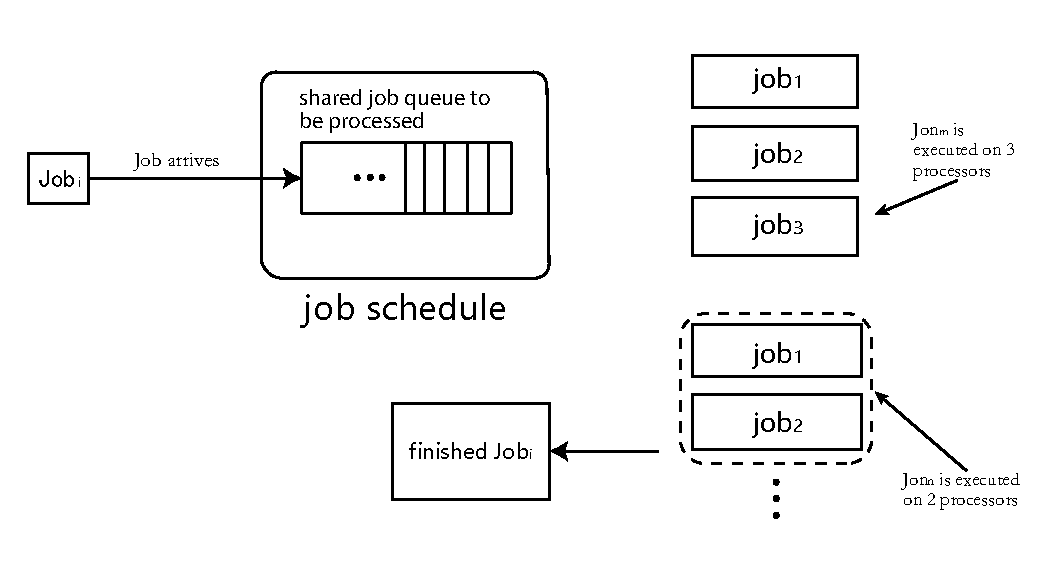
\includegraphics[height=0.45\textwidth]{52}
	\caption{作业调度模型}
	\label{fig-1}
\end{figure}

图\ref{fig-1}说明了本文假设的作业调度程序模型。在该图中,用户提交的作业到达共享作业队列,并且作业调度器获得作业请求的处理器的数量(job大小)。没有给作业调度程序提供其他信息。作业调度程序收集处理器的状态,空闲或忙碌,并将共享作业队列中的作业分派给空闲处理器。这里有两个执行作业的策略。在第一个策略中,作业调度程序将作业调度到S处理器,并保证在S处理器上执行作业直到完成。这里,S表示工作规模。在第二个策略中,作业调度程序不保证在S处理器上执行作业,也就是说,执行作业的处理器数量取决于并行计算机上作业的拥塞程度。在第一个策略中执行的作业称为刚性作业。

同时,一旦操作员处理了工作流程被实例化,它就被称为“任务”。实例化在调用抽象运算符时定义特定值,参数化任务成为DAG中的节点。基于该层处理,任务被分成几个部分,可以分派到服务器进行处理,这通常称为“任务实例”。任务实例表示任务的特定运行,其特征在于标记,任务和时间点的组合。由于流程的抽象和复杂性,图\ref{fig-2}向我们展示了如何作业实例将逐步拆分为任务实例。

\begin{figure}[htbp]
	\centering
	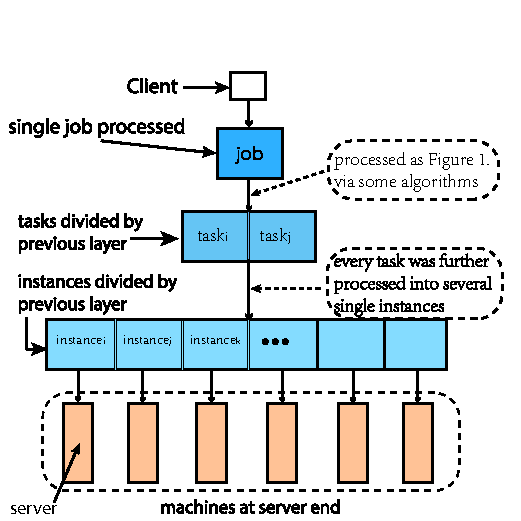
\includegraphics[height=0.55\textwidth]{5}
	\caption{来自作业层的工作流程型}
	\label{fig-2}
\end{figure}
\subsection{数据集分析}
本研究中使用的数据集cluster-trace-v2018\footnote{\ https://github.com/guanxyz/clusterdata/blob/master/cluster-trace-v2018/trace\_2018.md}将从我们的一个生产集群中进行跟踪和采样,cluster-trace-v2018是Alibaba Open Cluster Tracking Program\footnote{\ 阿里巴巴集群跟踪计划由阿里巴巴集团出版。通过提供来自实际生产的集群跟踪,该计划帮助研究人员,学生和对该领域感兴趣的人更好地了解现代互联网数据中心(IDC)和工作负载的特征。https://github.com/guanxyz/clusterdata}的一部分。该计划由阿里巴巴集团发布,并于2017年提出并开始跟踪。通过实际生产提供集群跟踪,该计划帮助研究人员,学生和对该领域感兴趣的人更好地了解现代互联网数据中心的功能和工作量(ID)。该项目目前已在Version 2017\footnote{\ https://github.com/guanxyz/clusterdata/tree/master/cluster-trace-v2017}和2018版本中提供。 2017版本是该程序的原型,它记录了3000个服务器节点的12小时跟踪。为了研究的全面性和完整性,我们打算在2018年版的基础上进行研究。cluster-trace-v2018包括大约4000台机器,跨时8天,由6个单独的数据文件组成,数据文件总大小达到了206GB,以下是该数据集的简要介绍:
\begin{itemize}
	\item machine\_meta:机器的元信息和事件信息。
	\item machine\_usage:每台机器的资源使用情况。
	\item containe\_meta:容器的元信息和事件信息。
	\item container\_usage:每个容器的资源使用情况。
	\item batch\_instance:有关批处理工作负载中实例的信息。
	\item batch\_task:有关批处理工作负载中实例的信息。
\end{itemize}

以上六个数据集在空间性上和时序性上向我们充分展示了每台服务器的信息、运行情况以及服务器所接受的任务调度,横向和纵向的展示了在为其8天的事件范围内所有任务的调度情况以及接受这些调度的机器的运行状态。
\section{关键问题}
\subsection{数据处理}
由于研究所采用的数据集十分庞大,故成为了本项目进行的一大难题。用以往的方法去分析和处理该数据集并不是最理想的手段,比如将整个数据读入内存然后进行处理,或者将数据按时序拆分成多个数据文件在单独进行处理。前者不可行的原因是实验地点的硬件条件还不能满足将如此庞大的数据这个整个读入内存,这必将造成计算机内存过载导致系统崩溃,而后者也不是最理想化的解决办法,因为比如将数据文件按天数切割成8份,每一份的文件大小也将达到15GB,即使可以读入内存但是也造成了内存占用率过高从而导致其他进程无法正常运行。

在另一方面来说,假设我们用某种方法将数据成功的导入了我们指定的数据库,但是在后台与数据库交互的过程中,由于查询的数据量过于庞大,会导致超出后台数据接口所能容纳的数据量最大限额,导致查询时间过慢或者因为超出接口限额请求时间过长而进程中断导致程序崩溃。

综上所述,以上两个难点都是因为数据量的规模所导致的问题,所以如何处理大数据量的数据集是本次项目亟待解决的一个难点。
\subsection{集群表示及定位故障源}
如何将任务(job)、作业(task)和作业实例(instance)(以下分别简称job、task和instance)与运行节点通过可视化手段巧妙地结合起来将成为一个有价值的话题。按照传统方法,先将所有节点与其运行状态在一个视图中表示出来,再通过交互使之与另一数据表中的job等参数链接起来,虽然可行但是再操作的过程中略显繁琐。而且根据数据文件的特征,决定了不能从节点使用情况的视图出发去查询作业实例等信息,两者的数据文件中的时间戳存在被包含的关系,所以不能用传统机械的方法去处理本项目的数据结构。

该关系可以大致归纳为一个树形结构,job、task与instance从前往后依次存在包含关系,而对于每一个instance都有一台独立的服务器节点用来处理该instance所发出的请求。该请求的分布可能是分布式的,这就导致了通一个job下所包含的instances被调度到了不同的节点来进行处理,所谓分布式任务调度。

值得注意的是,用户节点与job之间只存在一对多的关系,不存在不同用户所调度的job属于同一个job,这一点十分关键,在第三章第一节将具体分析此数据结构的特点。
\subsection{故障域算法}
用来判断硬件性能的算法不少,但是用于检测服务器负载异常的算法却不多见,而且使用范围有限。大规模服务器集群的异常确定算法类似于云计算基础设施中异常识别的处理模式。 该方法,最相关的主成分(MRPC)\footnote{\ Most relevant procedure component},由于缺乏动态规范化单位和规模的关键参数,因此无法应用于我们的研究。 
\subsection{时序性及空间性}
在研究目标为实时性的要求下,对时序性的反映往往是至关重要的。采用数据库的目的是可以实时对数据库内的记录进行可视化输出,然而这还远远不够,我们需要通过节点的过往记录和对未来节点运行状态的预测来具有时效性的描述节点,这样管理者不但可以从视图的渲染中找到异常规律从而在以后有针对性的操作节点,还可以对未来节点的运行状态进行预测,适当关闭或者限流问题节点从而对整个服务器集群和用户端的操作进行优化和改进。

在布局的空间性问题上,往往要在有限个数的可控维度上尽可能多的表示信息,所以节点的空间性排布成为一个值得商榷的问题。按照团队的初步设想,将节点表示为具有时序性的三维排布,每个维度各自表示判定异常的相关参数(CPU利用率、memory利用率、disk利用率),但这样做的成果其实并不理想:使用者并不关心每个节点的异常参数,所以对维度的利用是一种浪费,不符合可视分析的规范。